\documentclass[1p]{elsarticle_modified}
%\bibliographystyle{elsarticle-num}

%\usepackage[colorlinks]{hyperref}
%\usepackage{abbrmath_seonhwa} %\Abb, \Ascr, \Acal ,\Abf, \Afrak
\usepackage{amsfonts}
\usepackage{amssymb}
\usepackage{amsmath}
\usepackage{amsthm}
\usepackage{scalefnt}
\usepackage{amsbsy}
\usepackage{kotex}
\usepackage{caption}
\usepackage{subfig}
\usepackage{color}
\usepackage{graphicx}
\usepackage{xcolor} %% white, black, red, green, blue, cyan, magenta, yellow
\usepackage{float}
\usepackage{setspace}
\usepackage{hyperref}

\usepackage{tikz}
\usetikzlibrary{arrows}

\usepackage{multirow}
\usepackage{array} % fixed length table
\usepackage{hhline}

%%%%%%%%%%%%%%%%%%%%%
\makeatletter
\renewcommand*\env@matrix[1][\arraystretch]{%
	\edef\arraystretch{#1}%
	\hskip -\arraycolsep
	\let\@ifnextchar\new@ifnextchar
	\array{*\c@MaxMatrixCols c}}
\makeatother %https://tex.stackexchange.com/questions/14071/how-can-i-increase-the-line-spacing-in-a-matrix
%%%%%%%%%%%%%%%

\usepackage[normalem]{ulem}

\newcommand{\msout}[1]{\ifmmode\text{\sout{\ensuremath{#1}}}\else\sout{#1}\fi}
%SOURCE: \msout is \stkout macro in https://tex.stackexchange.com/questions/20609/strikeout-in-math-mode

\newcommand{\cancel}[1]{
	\ifmmode
	{\color{red}\msout{#1}}
	\else
	{\color{red}\sout{#1}}
	\fi
}

\newcommand{\add}[1]{
	{\color{blue}\uwave{#1}}
}

\newcommand{\replace}[2]{
	\ifmmode
	{\color{red}\msout{#1}}{\color{blue}\uwave{#2}}
	\else
	{\color{red}\sout{#1}}{\color{blue}\uwave{#2}}
	\fi
}

\newcommand{\Sol}{\mathcal{S}} %segment
\newcommand{\D}{D} %diagram
\newcommand{\A}{\mathcal{A}} %arc


%%%%%%%%%%%%%%%%%%%%%%%%%%%%%5 test

\def\sl{\operatorname{\textup{SL}}(2,\Cbb)}
\def\psl{\operatorname{\textup{PSL}}(2,\Cbb)}
\def\quan{\mkern 1mu \triangleright \mkern 1mu}

\theoremstyle{definition}
\newtheorem{thm}{Theorem}[section]
\newtheorem{prop}[thm]{Proposition}
\newtheorem{lem}[thm]{Lemma}
\newtheorem{ques}[thm]{Question}
\newtheorem{cor}[thm]{Corollary}
\newtheorem{defn}[thm]{Definition}
\newtheorem{exam}[thm]{Example}
\newtheorem{rmk}[thm]{Remark}
\newtheorem{alg}[thm]{Algorithm}

\newcommand{\I}{\sqrt{-1}}
\begin{document}

%\begin{frontmatter}
%
%\title{Boundary parabolic representations of knots up to 8 crossings}
%
%%% Group authors per affiliation:
%\author{Yunhi Cho} 
%\address{Department of Mathematics, University of Seoul, Seoul, Korea}
%\ead{yhcho@uos.ac.kr}
%
%
%\author{Seonhwa Kim} %\fnref{s_kim}}
%\address{Center for Geometry and Physics, Institute for Basic Science, Pohang, 37673, Korea}
%\ead{ryeona17@ibs.re.kr}
%
%\author{Hyuk Kim}
%\address{Department of Mathematical Sciences, Seoul National University, Seoul 08826, Korea}
%\ead{hyukkim@snu.ac.kr}
%
%\author{Seokbeom Yoon}
%\address{Department of Mathematical Sciences, Seoul National University, Seoul, 08826,  Korea}
%\ead{sbyoon15@snu.ac.kr}
%
%\begin{abstract}
%We find all boundary parabolic representation of knots up to 8 crossings.
%
%\end{abstract}
%\begin{keyword}
%    \MSC[2010] 57M25 
%\end{keyword}
%
%\end{frontmatter}

%\linenumbers
%\tableofcontents
%
\newcommand\colored[1]{\textcolor{white}{\rule[-0.35ex]{0.8em}{1.4ex}}\kern-0.8em\color{red} #1}%
%\newcommand\colored[1]{\textcolor{white}{ #1}\kern-2.17ex	\textcolor{white}{ #1}\kern-1.81ex	\textcolor{white}{ #1}\kern-2.15ex\color{red}#1	}

{\Large $\underline{12n_{0086}~(K12n_{0086})}$}

\setlength{\tabcolsep}{10pt}
\renewcommand{\arraystretch}{1.6}
\vspace{1cm}\begin{tabular}{m{100pt}>{\centering\arraybackslash}m{274pt}}
\multirow{5}{120pt}{
	\centering
	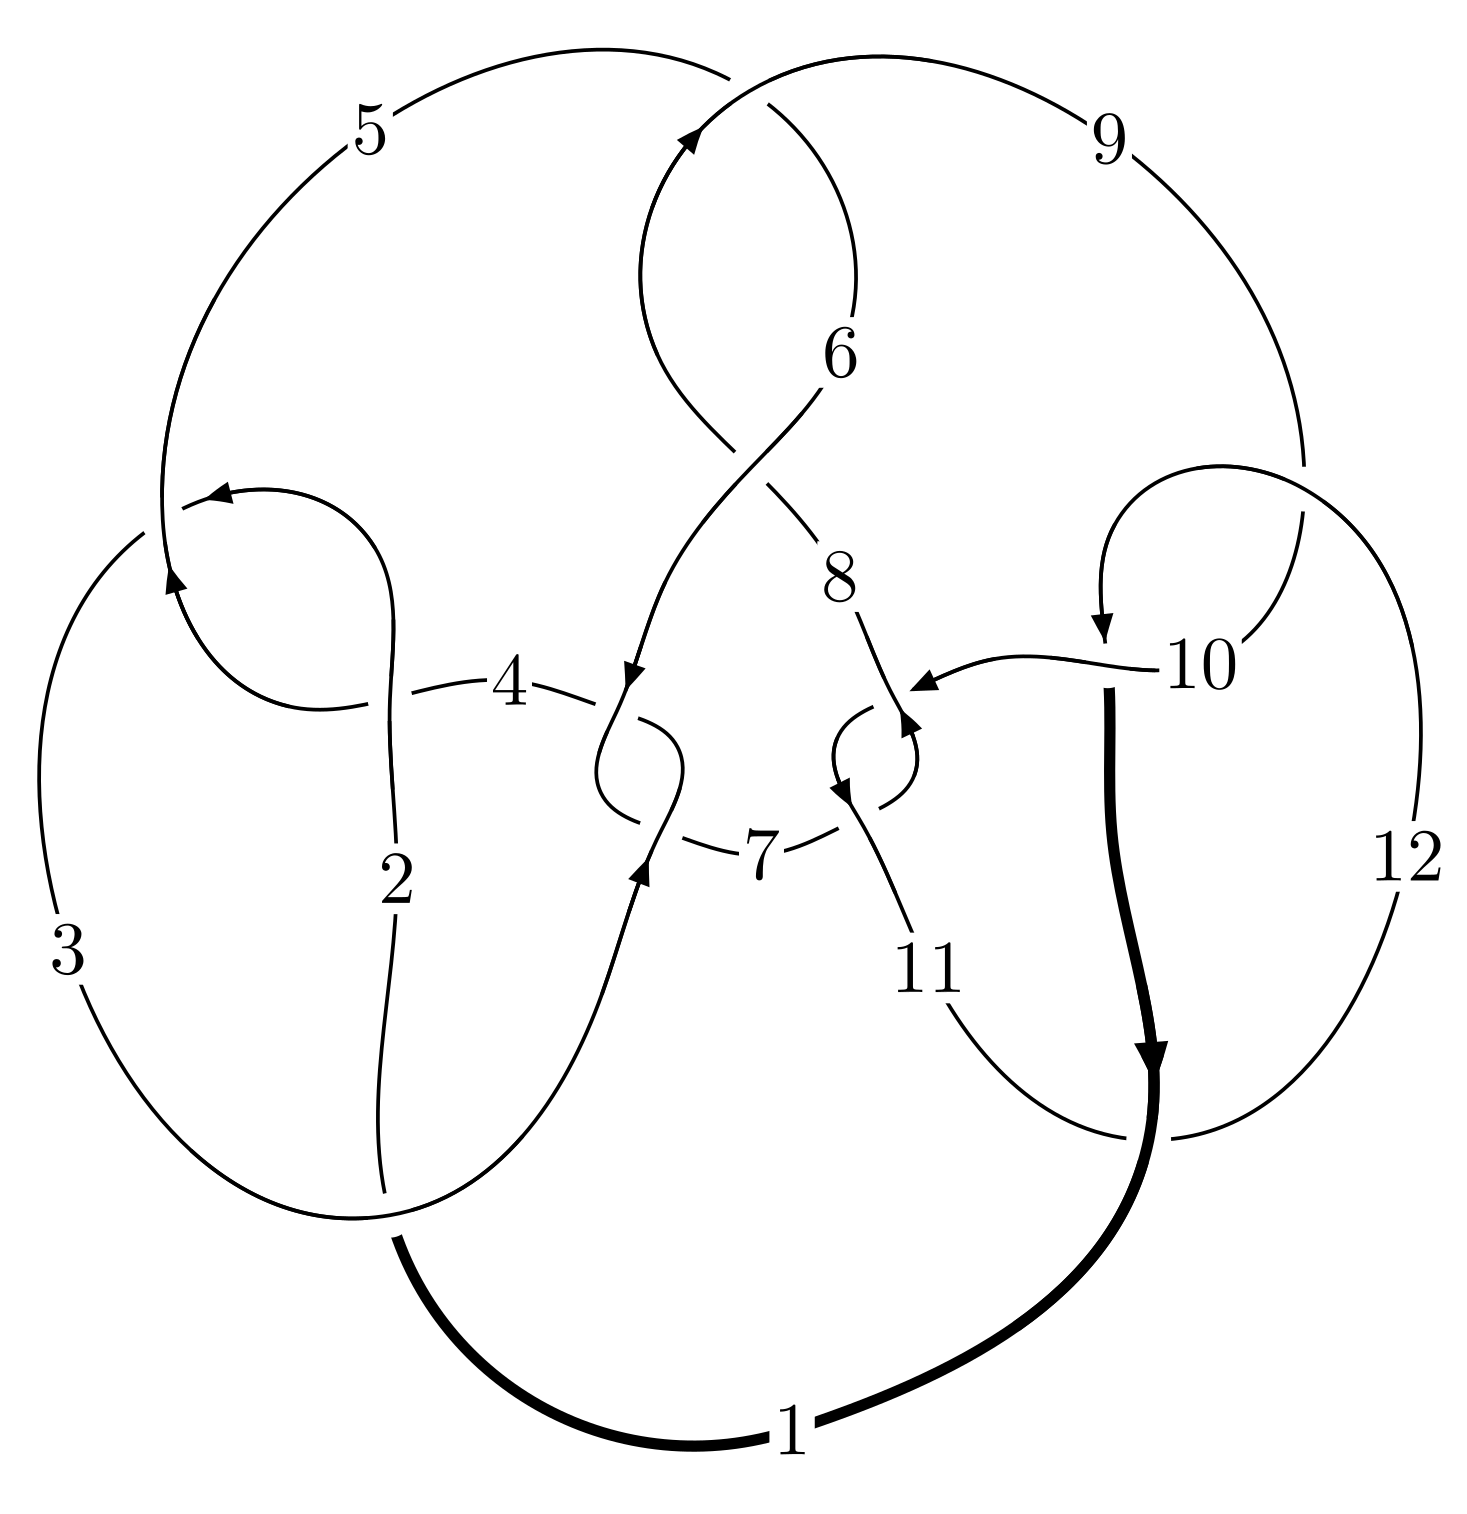
\includegraphics[width=112pt]{../../../GIT/diagram.site/Diagrams/png/2175_12n_0086.png}\\
\ \ \ A knot diagram\footnotemark}&
\allowdisplaybreaks
\textbf{Linearized knot diagam} \\
\cline{2-2}
 &
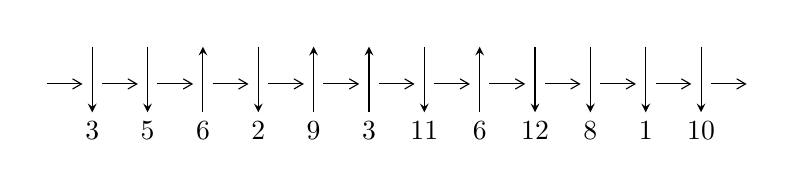
\begin{tikzpicture}[x=20pt, y=17pt]
	% nodes
	\node (C0) at (0, 0) {};
	\node (C1) at (1, 0) {};
	\node (C1U) at (1, +1) {};
	\node (C1D) at (1, -1) {3};

	\node (C2) at (2, 0) {};
	\node (C2U) at (2, +1) {};
	\node (C2D) at (2, -1) {5};

	\node (C3) at (3, 0) {};
	\node (C3U) at (3, +1) {};
	\node (C3D) at (3, -1) {6};

	\node (C4) at (4, 0) {};
	\node (C4U) at (4, +1) {};
	\node (C4D) at (4, -1) {2};

	\node (C5) at (5, 0) {};
	\node (C5U) at (5, +1) {};
	\node (C5D) at (5, -1) {9};

	\node (C6) at (6, 0) {};
	\node (C6U) at (6, +1) {};
	\node (C6D) at (6, -1) {3};

	\node (C7) at (7, 0) {};
	\node (C7U) at (7, +1) {};
	\node (C7D) at (7, -1) {11};

	\node (C8) at (8, 0) {};
	\node (C8U) at (8, +1) {};
	\node (C8D) at (8, -1) {6};

	\node (C9) at (9, 0) {};
	\node (C9U) at (9, +1) {};
	\node (C9D) at (9, -1) {12};

	\node (C10) at (10, 0) {};
	\node (C10U) at (10, +1) {};
	\node (C10D) at (10, -1) {8};

	\node (C11) at (11, 0) {};
	\node (C11U) at (11, +1) {};
	\node (C11D) at (11, -1) {1};

	\node (C12) at (12, 0) {};
	\node (C12U) at (12, +1) {};
	\node (C12D) at (12, -1) {10};
	\node (C13) at (13, 0) {};

	% arrows
	\draw[->,>={angle 60}]
	(C0) edge (C1) (C1) edge (C2) (C2) edge (C3) (C3) edge (C4) (C4) edge (C5) (C5) edge (C6) (C6) edge (C7) (C7) edge (C8) (C8) edge (C9) (C9) edge (C10) (C10) edge (C11) (C11) edge (C12) (C12) edge (C13) ;	\draw[->,>=stealth]
	(C1U) edge (C1D) (C2U) edge (C2D) (C3D) edge (C3U) (C4U) edge (C4D) (C5D) edge (C5U) (C6D) edge (C6U) (C7U) edge (C7D) (C8D) edge (C8U) (C9U) edge (C9D) (C10U) edge (C10D) (C11U) edge (C11D) (C12U) edge (C12D) ;
	\end{tikzpicture} \\
\hhline{~~} \\& 
\textbf{Solving Sequence} \\ \cline{2-2} 
 &
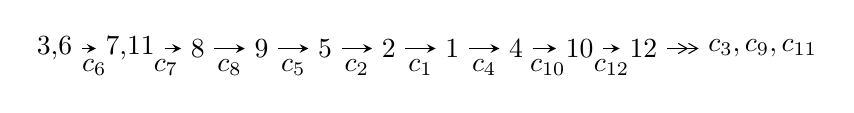
\begin{tikzpicture}[x=23pt, y=7pt]
	% node
	\node (A0) at (-1/8, 0) {3,6};
	\node (A1) at (17/16, 0) {7,11};
	\node (A2) at (17/8, 0) {8};
	\node (A3) at (25/8, 0) {9};
	\node (A4) at (33/8, 0) {5};
	\node (A5) at (41/8, 0) {2};
	\node (A6) at (49/8, 0) {1};
	\node (A7) at (57/8, 0) {4};
	\node (A8) at (65/8, 0) {10};
	\node (A9) at (73/8, 0) {12};
	\node (C1) at (1/2, -1) {$c_{6}$};
	\node (C2) at (13/8, -1) {$c_{7}$};
	\node (C3) at (21/8, -1) {$c_{8}$};
	\node (C4) at (29/8, -1) {$c_{5}$};
	\node (C5) at (37/8, -1) {$c_{2}$};
	\node (C6) at (45/8, -1) {$c_{1}$};
	\node (C7) at (53/8, -1) {$c_{4}$};
	\node (C8) at (61/8, -1) {$c_{10}$};
	\node (C9) at (69/8, -1) {$c_{12}$};
	\node (A10) at (11, 0) {$c_{3},c_{9},c_{11}$};

	% edge
	\draw[->,>=stealth]	
	(A0) edge (A1) (A1) edge (A2) (A2) edge (A3) (A3) edge (A4) (A4) edge (A5) (A5) edge (A6) (A6) edge (A7) (A7) edge (A8) (A8) edge (A9) ;
	\draw[->>,>={angle 60}]	
	(A9) edge (A10);
\end{tikzpicture} \\ 

\end{tabular} \\

\footnotetext{
The image of knot diagram is generated by the software ``\textbf{Draw programme}" developed by Andrew Bartholomew(\url{http://www.layer8.co.uk/maths/draw/index.htm\#Running-draw}), where we modified some parts for our purpose(\url{https://github.com/CATsTAILs/LinksPainter}).
}\phantom \\ \newline 
\centering \textbf{Ideals for irreducible components\footnotemark of $X_{\text{par}}$} 
 
\begin{align*}
I^u_{1}&=\langle 
1.19780\times10^{241} u^{65}+8.81073\times10^{241} u^{64}+\cdots+3.02569\times10^{240} b+9.53394\times10^{243},\\
\phantom{I^u_{1}}&\phantom{= \langle  }8.96655\times10^{240} u^{65}+6.61765\times10^{241} u^{64}+\cdots+3.02569\times10^{240} a+6.94724\times10^{243},\\
\phantom{I^u_{1}}&\phantom{= \langle  }u^{66}+8 u^{65}+\cdots-7168 u+512\rangle \\
I^u_{2}&=\langle 
u^5-2 u^3- u^2+b+2 u+1,\;u^5+2 u^4- u^3-3 u^2+a+2,\;u^6+u^5- u^4-2 u^3+u+1\rangle \\
\\
I^v_{1}&=\langle 
a,\;1742 v^8-24207 v^7-17107 v^6+21829 v^5+12682 v^4-26226 v^3-24997 v^2+683 b-5624 v+648,\\
\phantom{I^v_{1}}&\phantom{= \langle  }v^9-13 v^8-22 v^7+15 v^5-5 v^4-25 v^3-20 v^2-7 v-1\rangle \\
\end{align*}
\raggedright * 3 irreducible components of $\dim_{\mathbb{C}}=0$, with total 81 representations.\\
\footnotetext{All coefficients of polynomials are rational numbers. But the coefficients are sometimes approximated in decimal forms when there is not enough margin.}
\newpage
\renewcommand{\arraystretch}{1}
\centering \section*{I. $I^u_{1}= \langle 1.20\times10^{241} u^{65}+8.81\times10^{241} u^{64}+\cdots+3.03\times10^{240} b+9.53\times10^{243},\;8.97\times10^{240} u^{65}+6.62\times10^{241} u^{64}+\cdots+3.03\times10^{240} a+6.95\times10^{243},\;u^{66}+8 u^{65}+\cdots-7168 u+512 \rangle$}
\flushleft \textbf{(i) Arc colorings}\\
\begin{tabular}{m{7pt} m{180pt} m{7pt} m{180pt} }
\flushright $a_{3}=$&$\begin{pmatrix}0\\u\end{pmatrix}$ \\
\flushright $a_{6}=$&$\begin{pmatrix}1\\0\end{pmatrix}$ \\
\flushright $a_{7}=$&$\begin{pmatrix}1\\- u^2\end{pmatrix}$ \\
\flushright $a_{11}=$&$\begin{pmatrix}-2.96348 u^{65}-21.8716 u^{64}+\cdots+37209.0 u-2296.09\\-3.95876 u^{65}-29.1198 u^{64}+\cdots+48993.3 u-3151.00\end{pmatrix}$ \\
\flushright $a_{8}=$&$\begin{pmatrix}-0.189192 u^{65}-1.42917 u^{64}+\cdots+3725.71 u-278.930\\-3.64017 u^{65}-26.9641 u^{64}+\cdots+48969.5 u-3124.72\end{pmatrix}$ \\
\flushright $a_{9}=$&$\begin{pmatrix}-3.82936 u^{65}-28.3933 u^{64}+\cdots+52695.2 u-3403.65\\-3.64017 u^{65}-26.9641 u^{64}+\cdots+48969.5 u-3124.72\end{pmatrix}$ \\
\flushright $a_{5}=$&$\begin{pmatrix}-0.597599 u^{65}-4.38854 u^{64}+\cdots+7145.50 u-452.205\\-1.29177 u^{65}-9.48251 u^{64}+\cdots+15607.1 u-1005.22\end{pmatrix}$ \\
\flushright $a_{2}=$&$\begin{pmatrix}-0.694167 u^{65}-5.09397 u^{64}+\cdots+8461.64 u-553.013\\-1.29177 u^{65}-9.48251 u^{64}+\cdots+15607.1 u-1005.22\end{pmatrix}$ \\
\flushright $a_{1}=$&$\begin{pmatrix}-0.694167 u^{65}-5.09397 u^{64}+\cdots+8461.64 u-553.013\\-0.988463 u^{65}-7.25680 u^{64}+\cdots+11959.0 u-770.026\end{pmatrix}$ \\
\flushright $a_{4}=$&$\begin{pmatrix}u\\u\end{pmatrix}$ \\
\flushright $a_{10}=$&$\begin{pmatrix}-3.85958 u^{65}-28.4537 u^{64}+\cdots+47856.5 u-2957.77\\-7.03239 u^{65}-51.8312 u^{64}+\cdots+89324.7 u-5730.22\end{pmatrix}$ \\
\flushright $a_{12}=$&$\begin{pmatrix}-4.70834 u^{65}-34.8004 u^{64}+\cdots+60886.6 u-3811.37\\-7.53902 u^{65}-55.6488 u^{64}+\cdots+97468.3 u-6242.36\end{pmatrix}$\\&\end{tabular}
\flushleft \textbf{(ii) Obstruction class $= -1$}\\~\\
\flushleft \textbf{(iii) Cusp Shapes $= 12.0986 u^{65}+88.8600 u^{64}+\cdots-142679. u+8879.59$}\\~\\
\newpage\renewcommand{\arraystretch}{1}
\flushleft \textbf{(iv) u-Polynomials at the component}\newline \\
\begin{tabular}{m{50pt}|m{274pt}}
Crossings & \hspace{64pt}u-Polynomials at each crossing \\
\hline $$\begin{aligned}c_{1}\end{aligned}$$&$\begin{aligned}
&u^{66}+21 u^{65}+\cdots+31524 u+1
\end{aligned}$\\
\hline $$\begin{aligned}c_{2},c_{4}\end{aligned}$$&$\begin{aligned}
&u^{66}-11 u^{65}+\cdots+184 u-1
\end{aligned}$\\
\hline $$\begin{aligned}c_{3},c_{6}\end{aligned}$$&$\begin{aligned}
&u^{66}+8 u^{65}+\cdots-7168 u+512
\end{aligned}$\\
\hline $$\begin{aligned}c_{5},c_{8}\end{aligned}$$&$\begin{aligned}
&u^{66}+3 u^{65}+\cdots-2 u-1
\end{aligned}$\\
\hline $$\begin{aligned}c_{7},c_{10}\end{aligned}$$&$\begin{aligned}
&u^{66}-2 u^{65}+\cdots+192 u+64
\end{aligned}$\\
\hline $$\begin{aligned}c_{9},c_{12}\end{aligned}$$&$\begin{aligned}
&u^{66}-8 u^{65}+\cdots-11 u+1
\end{aligned}$\\
\hline $$\begin{aligned}c_{11}\end{aligned}$$&$\begin{aligned}
&u^{66}+28 u^{65}+\cdots-143 u+1
\end{aligned}$\\
\hline
\end{tabular}\\~\\
\newpage\renewcommand{\arraystretch}{1}
\flushleft \textbf{(v) Riley Polynomials at the component}\newline \\
\begin{tabular}{m{50pt}|m{274pt}}
Crossings & \hspace{64pt}Riley Polynomials at each crossing \\
\hline $$\begin{aligned}c_{1}\end{aligned}$$&$\begin{aligned}
&y^{66}+59 y^{65}+\cdots-992297680 y+1
\end{aligned}$\\
\hline $$\begin{aligned}c_{2},c_{4}\end{aligned}$$&$\begin{aligned}
&y^{66}-21 y^{65}+\cdots-31524 y+1
\end{aligned}$\\
\hline $$\begin{aligned}c_{3},c_{6}\end{aligned}$$&$\begin{aligned}
&y^{66}-60 y^{65}+\cdots-76021760 y+262144
\end{aligned}$\\
\hline $$\begin{aligned}c_{5},c_{8}\end{aligned}$$&$\begin{aligned}
&y^{66}+15 y^{65}+\cdots-20 y+1
\end{aligned}$\\
\hline $$\begin{aligned}c_{7},c_{10}\end{aligned}$$&$\begin{aligned}
&y^{66}+42 y^{65}+\cdots+77824 y+4096
\end{aligned}$\\
\hline $$\begin{aligned}c_{9},c_{12}\end{aligned}$$&$\begin{aligned}
&y^{66}-28 y^{65}+\cdots+143 y+1
\end{aligned}$\\
\hline $$\begin{aligned}c_{11}\end{aligned}$$&$\begin{aligned}
&y^{66}+28 y^{65}+\cdots-12229 y+1
\end{aligned}$\\
\hline
\end{tabular}\\~\\
\newpage\flushleft \textbf{(vi) Complex Volumes and Cusp Shapes}
$$\begin{array}{c|c|c}  
\text{Solutions to }I^u_{1}& \I (\text{vol} + \sqrt{-1}CS) & \text{Cusp shape}\\
 \hline 
\begin{aligned}
u &= -0.896621 + 0.222919 I \\
a &= -0.68390 + 2.68834 I \\
b &= -0.03058 - 1.93558 I\end{aligned}
 & -4.31795 + 0.78820 I & \phantom{-0.000000 } 0 \\ \hline\begin{aligned}
u &= -0.896621 - 0.222919 I \\
a &= -0.68390 - 2.68834 I \\
b &= -0.03058 + 1.93558 I\end{aligned}
 & -4.31795 - 0.78820 I & \phantom{-0.000000 } 0 \\ \hline\begin{aligned}
u &= -0.161444 + 0.873142 I \\
a &= \phantom{-}0.24159 - 2.29188 I \\
b &= \phantom{-}0.96672 - 2.19128 I\end{aligned}
 & -3.21013 + 1.26950 I & \phantom{-0.000000 } 0 \\ \hline\begin{aligned}
u &= -0.161444 - 0.873142 I \\
a &= \phantom{-}0.24159 + 2.29188 I \\
b &= \phantom{-}0.96672 + 2.19128 I\end{aligned}
 & -3.21013 - 1.26950 I & \phantom{-0.000000 } 0 \\ \hline\begin{aligned}
u &= \phantom{-}0.734614 + 0.498569 I \\
a &= -0.296201 + 0.045995 I \\
b &= \phantom{-}0.216817 + 0.815085 I\end{aligned}
 & \phantom{-}1.31523 + 1.27199 I & \phantom{-0.000000 } 0 \\ \hline\begin{aligned}
u &= \phantom{-}0.734614 - 0.498569 I \\
a &= -0.296201 - 0.045995 I \\
b &= \phantom{-}0.216817 - 0.815085 I\end{aligned}
 & \phantom{-}1.31523 - 1.27199 I & \phantom{-0.000000 } 0 \\ \hline\begin{aligned}
u &= \phantom{-}0.015880 + 1.156380 I \\
a &= -1.200970 + 0.600425 I \\
b &= -0.773578 + 1.087150 I\end{aligned}
 & -2.23471 + 2.98196 I & \phantom{-0.000000 } 0 \\ \hline\begin{aligned}
u &= \phantom{-}0.015880 - 1.156380 I \\
a &= -1.200970 - 0.600425 I \\
b &= -0.773578 - 1.087150 I\end{aligned}
 & -2.23471 - 2.98196 I & \phantom{-0.000000 } 0 \\ \hline\begin{aligned}
u &= \phantom{-}0.043693 + 0.829853 I \\
a &= \phantom{-}1.154180 + 0.810143 I \\
b &= \phantom{-}0.493220 - 0.823559 I\end{aligned}
 & \phantom{-}2.07274 - 4.10478 I & \phantom{-0.000000 } 0 \\ \hline\begin{aligned}
u &= \phantom{-}0.043693 - 0.829853 I \\
a &= \phantom{-}1.154180 - 0.810143 I \\
b &= \phantom{-}0.493220 + 0.823559 I\end{aligned}
 & \phantom{-}2.07274 + 4.10478 I & \phantom{-0.000000 } 0\\
 \hline 
 \end{array}$$\newpage$$\begin{array}{c|c|c}  
\text{Solutions to }I^u_{1}& \I (\text{vol} + \sqrt{-1}CS) & \text{Cusp shape}\\
 \hline 
\begin{aligned}
u &= -1.010290 + 0.635704 I \\
a &= \phantom{-}0.0712092 - 0.0097906 I \\
b &= \phantom{-}0.045899 - 0.458605 I\end{aligned}
 & -1.20228 - 5.48361 I & \phantom{-0.000000 } 0 \\ \hline\begin{aligned}
u &= -1.010290 - 0.635704 I \\
a &= \phantom{-}0.0712092 + 0.0097906 I \\
b &= \phantom{-}0.045899 + 0.458605 I\end{aligned}
 & -1.20228 + 5.48361 I & \phantom{-0.000000 } 0 \\ \hline\begin{aligned}
u &= -0.178380 + 0.763029 I \\
a &= -1.123200 - 0.224763 I \\
b &= -0.584767 + 0.854259 I\end{aligned}
 & \phantom{-}2.74552 + 1.51786 I & \phantom{-0.000000 } 0 \\ \hline\begin{aligned}
u &= -0.178380 - 0.763029 I \\
a &= -1.123200 + 0.224763 I \\
b &= -0.584767 - 0.854259 I\end{aligned}
 & \phantom{-}2.74552 - 1.51786 I & \phantom{-0.000000 } 0 \\ \hline\begin{aligned}
u &= \phantom{-}0.710476 + 0.000507 I \\
a &= -0.047677 + 0.256353 I \\
b &= -0.191197 - 0.906715 I\end{aligned}
 & \phantom{-}1.17931 - 1.63015 I & \phantom{-0.000000 -}0. + 3.30141 I \\ \hline\begin{aligned}
u &= \phantom{-}0.710476 - 0.000507 I \\
a &= -0.047677 - 0.256353 I \\
b &= -0.191197 + 0.906715 I\end{aligned}
 & \phantom{-}1.17931 + 1.63015 I & \phantom{-0.000000 } 0. - 3.30141 I \\ \hline\begin{aligned}
u &= -0.438003 + 0.525280 I \\
a &= -1.44839 - 0.54246 I \\
b &= -0.083240 - 0.461268 I\end{aligned}
 & -1.91057 + 0.79816 I & -4.00000 + 0. I\phantom{ +0.000000I} \\ \hline\begin{aligned}
u &= -0.438003 - 0.525280 I \\
a &= -1.44839 + 0.54246 I \\
b &= -0.083240 + 0.461268 I\end{aligned}
 & -1.91057 - 0.79816 I & -4.00000 + 0. I\phantom{ +0.000000I} \\ \hline\begin{aligned}
u &= -0.681040 + 0.017244 I \\
a &= \phantom{-}0.147299 - 0.561967 I \\
b &= -0.847666 - 0.591726 I\end{aligned}
 & -1.43375 - 2.91518 I & \phantom{-0.000000 -}0. + 4.85019 I \\ \hline\begin{aligned}
u &= -0.681040 - 0.017244 I \\
a &= \phantom{-}0.147299 + 0.561967 I \\
b &= -0.847666 + 0.591726 I\end{aligned}
 & -1.43375 + 2.91518 I & \phantom{-0.000000 } 0. - 4.85019 I\\
 \hline 
 \end{array}$$\newpage$$\begin{array}{c|c|c}  
\text{Solutions to }I^u_{1}& \I (\text{vol} + \sqrt{-1}CS) & \text{Cusp shape}\\
 \hline 
\begin{aligned}
u &= -0.006104 + 0.635645 I \\
a &= \phantom{-}1.91287 - 1.80281 I \\
b &= \phantom{-}0.052848 - 0.610826 I\end{aligned}
 & -1.82059 - 0.01526 I & -7.87182 + 0.48568 I \\ \hline\begin{aligned}
u &= -0.006104 - 0.635645 I \\
a &= \phantom{-}1.91287 + 1.80281 I \\
b &= \phantom{-}0.052848 + 0.610826 I\end{aligned}
 & -1.82059 + 0.01526 I & -7.87182 - 0.48568 I \\ \hline\begin{aligned}
u &= -0.619648 + 0.008490 I \\
a &= -0.511507 - 0.814092 I \\
b &= \phantom{-}1.051820 - 0.516985 I\end{aligned}
 & -5.23148 - 1.44469 I & -2.19147 + 1.36304 I \\ \hline\begin{aligned}
u &= -0.619648 - 0.008490 I \\
a &= -0.511507 + 0.814092 I \\
b &= \phantom{-}1.051820 + 0.516985 I\end{aligned}
 & -5.23148 + 1.44469 I & -2.19147 - 1.36304 I \\ \hline\begin{aligned}
u &= -0.598433 + 0.144408 I \\
a &= -0.338653 + 0.326080 I \\
b &= \phantom{-}0.823727 + 0.764068 I\end{aligned}
 & -4.86194 - 7.45999 I & -0.96246 + 11.41011 I \\ \hline\begin{aligned}
u &= -0.598433 - 0.144408 I \\
a &= -0.338653 - 0.326080 I \\
b &= \phantom{-}0.823727 - 0.764068 I\end{aligned}
 & -4.86194 + 7.45999 I & -0.96246 - 11.41011 I \\ \hline\begin{aligned}
u &= \phantom{-}0.557706 + 0.143081 I \\
a &= \phantom{-}2.02290 + 5.39960 I \\
b &= \phantom{-}0.061106 - 0.673706 I\end{aligned}
 & \phantom{-}0.81136 + 2.64313 I & \phantom{-}13.7570 - 9.2546 I \\ \hline\begin{aligned}
u &= \phantom{-}0.557706 - 0.143081 I \\
a &= \phantom{-}2.02290 - 5.39960 I \\
b &= \phantom{-}0.061106 + 0.673706 I\end{aligned}
 & \phantom{-}0.81136 - 2.64313 I & \phantom{-}13.7570 + 9.2546 I \\ \hline\begin{aligned}
u &= \phantom{-}1.47897 + 0.04915 I \\
a &= \phantom{-}0.36193 - 1.79756 I \\
b &= -1.17938 + 2.79473 I\end{aligned}
 & \phantom{-}2.17496 + 0.19887 I & \phantom{-0.000000 } 0 \\ \hline\begin{aligned}
u &= \phantom{-}1.47897 - 0.04915 I \\
a &= \phantom{-}0.36193 + 1.79756 I \\
b &= -1.17938 - 2.79473 I\end{aligned}
 & \phantom{-}2.17496 - 0.19887 I & \phantom{-0.000000 } 0\\
 \hline 
 \end{array}$$\newpage$$\begin{array}{c|c|c}  
\text{Solutions to }I^u_{1}& \I (\text{vol} + \sqrt{-1}CS) & \text{Cusp shape}\\
 \hline 
\begin{aligned}
u &= \phantom{-}1.49869 + 0.12364 I \\
a &= \phantom{-}0.028754 + 0.149012 I \\
b &= -1.196520 - 0.662560 I\end{aligned}
 & \phantom{-}3.57906 + 2.47635 I & \phantom{-0.000000 } 0 \\ \hline\begin{aligned}
u &= \phantom{-}1.49869 - 0.12364 I \\
a &= \phantom{-}0.028754 - 0.149012 I \\
b &= -1.196520 + 0.662560 I\end{aligned}
 & \phantom{-}3.57906 - 2.47635 I & \phantom{-0.000000 } 0 \\ \hline\begin{aligned}
u &= -1.51285 + 0.03928 I \\
a &= \phantom{-}0.346340 - 1.327240 I \\
b &= -1.21560 + 1.60059 I\end{aligned}
 & \phantom{-}7.72304 - 2.79945 I & \phantom{-0.000000 } 0 \\ \hline\begin{aligned}
u &= -1.51285 - 0.03928 I \\
a &= \phantom{-}0.346340 + 1.327240 I \\
b &= -1.21560 - 1.60059 I\end{aligned}
 & \phantom{-}7.72304 + 2.79945 I & \phantom{-0.000000 } 0 \\ \hline\begin{aligned}
u &= -1.47811 + 0.34080 I \\
a &= -0.1005600 - 0.0917447 I \\
b &= -0.972026 + 0.012478 I\end{aligned}
 & \phantom{-}3.17239 - 3.89822 I & \phantom{-0.000000 } 0 \\ \hline\begin{aligned}
u &= -1.47811 - 0.34080 I \\
a &= -0.1005600 + 0.0917447 I \\
b &= -0.972026 - 0.012478 I\end{aligned}
 & \phantom{-}3.17239 + 3.89822 I & \phantom{-0.000000 } 0 \\ \hline\begin{aligned}
u &= -1.46366 + 0.47734 I \\
a &= -0.26778 + 1.74931 I \\
b &= -1.79456 - 2.53218 I\end{aligned}
 & \phantom{-}1.18870 - 6.56344 I & \phantom{-0.000000 } 0 \\ \hline\begin{aligned}
u &= -1.46366 - 0.47734 I \\
a &= -0.26778 - 1.74931 I \\
b &= -1.79456 + 2.53218 I\end{aligned}
 & \phantom{-}1.18870 + 6.56344 I & \phantom{-0.000000 } 0 \\ \hline\begin{aligned}
u &= \phantom{-}1.47312 + 0.46657 I \\
a &= \phantom{-}0.767438 + 1.139500 I \\
b &= -0.63144 - 1.94704 I\end{aligned}
 & \phantom{-}6.78475 + 9.23321 I & \phantom{-0.000000 } 0 \\ \hline\begin{aligned}
u &= \phantom{-}1.47312 - 0.46657 I \\
a &= \phantom{-}0.767438 - 1.139500 I \\
b &= -0.63144 + 1.94704 I\end{aligned}
 & \phantom{-}6.78475 - 9.23321 I & \phantom{-0.000000 } 0\\
 \hline 
 \end{array}$$\newpage$$\begin{array}{c|c|c}  
\text{Solutions to }I^u_{1}& \I (\text{vol} + \sqrt{-1}CS) & \text{Cusp shape}\\
 \hline 
\begin{aligned}
u &= \phantom{-}0.45244 + 1.51129 I \\
a &= \phantom{-}0.073063 + 0.503097 I \\
b &= \phantom{-}0.72561 + 2.13556 I\end{aligned}
 & \phantom{-}2.19847 + 2.32521 I & \phantom{-0.000000 } 0 \\ \hline\begin{aligned}
u &= \phantom{-}0.45244 - 1.51129 I \\
a &= \phantom{-}0.073063 - 0.503097 I \\
b &= \phantom{-}0.72561 - 2.13556 I\end{aligned}
 & \phantom{-}2.19847 - 2.32521 I & \phantom{-0.000000 } 0 \\ \hline\begin{aligned}
u &= \phantom{-}1.60960 + 0.20036 I \\
a &= -0.031037 + 0.149711 I \\
b &= \phantom{-}1.349420 - 0.252092 I\end{aligned}
 & \phantom{-}4.03833 + 2.66127 I & \phantom{-0.000000 } 0 \\ \hline\begin{aligned}
u &= \phantom{-}1.60960 - 0.20036 I \\
a &= -0.031037 - 0.149711 I \\
b &= \phantom{-}1.349420 + 0.252092 I\end{aligned}
 & \phantom{-}4.03833 - 2.66127 I & \phantom{-0.000000 } 0 \\ \hline\begin{aligned}
u &= -1.62095 + 0.14520 I \\
a &= -0.146836 - 1.371110 I \\
b &= \phantom{-}1.32921 + 1.94937 I\end{aligned}
 & \phantom{-}9.29382 - 3.78649 I & \phantom{-0.000000 } 0 \\ \hline\begin{aligned}
u &= -1.62095 - 0.14520 I \\
a &= -0.146836 + 1.371110 I \\
b &= \phantom{-}1.32921 - 1.94937 I\end{aligned}
 & \phantom{-}9.29382 + 3.78649 I & \phantom{-0.000000 } 0 \\ \hline\begin{aligned}
u &= -1.52811 + 0.57582 I \\
a &= \phantom{-}0.0964491 + 0.0666214 I \\
b &= \phantom{-}0.958300 - 0.287281 I\end{aligned}
 & \phantom{-}2.66554 - 9.42263 I & \phantom{-0.000000 } 0 \\ \hline\begin{aligned}
u &= -1.52811 - 0.57582 I \\
a &= \phantom{-}0.0964491 - 0.0666214 I \\
b &= \phantom{-}0.958300 + 0.287281 I\end{aligned}
 & \phantom{-}2.66554 + 9.42263 I & \phantom{-0.000000 } 0 \\ \hline\begin{aligned}
u &= \phantom{-}1.61436 + 0.32070 I \\
a &= -0.579677 - 1.239460 I \\
b &= \phantom{-}0.64699 + 2.29322 I\end{aligned}
 & \phantom{-}8.98485 + 3.05406 I & \phantom{-0.000000 } 0 \\ \hline\begin{aligned}
u &= \phantom{-}1.61436 - 0.32070 I \\
a &= -0.579677 + 1.239460 I \\
b &= \phantom{-}0.64699 - 2.29322 I\end{aligned}
 & \phantom{-}8.98485 - 3.05406 I & \phantom{-0.000000 } 0\\
 \hline 
 \end{array}$$\newpage$$\begin{array}{c|c|c}  
\text{Solutions to }I^u_{1}& \I (\text{vol} + \sqrt{-1}CS) & \text{Cusp shape}\\
 \hline 
\begin{aligned}
u &= -1.17931 + 1.15054 I \\
a &= -0.565320 + 0.704718 I \\
b &= -1.72394 - 0.50610 I\end{aligned}
 & -1.42259 - 0.46359 I & \phantom{-0.000000 } 0 \\ \hline\begin{aligned}
u &= -1.17931 - 1.15054 I \\
a &= -0.565320 - 0.704718 I \\
b &= -1.72394 + 0.50610 I\end{aligned}
 & -1.42259 + 0.46359 I & \phantom{-0.000000 } 0 \\ \hline\begin{aligned}
u &= -1.56100 + 0.72853 I \\
a &= \phantom{-}0.337392 - 0.874324 I \\
b &= \phantom{-}1.67630 + 1.29876 I\end{aligned}
 & -1.87995 + 4.31692 I & \phantom{-0.000000 } 0 \\ \hline\begin{aligned}
u &= -1.56100 - 0.72853 I \\
a &= \phantom{-}0.337392 + 0.874324 I \\
b &= \phantom{-}1.67630 - 1.29876 I\end{aligned}
 & -1.87995 - 4.31692 I & \phantom{-0.000000 } 0 \\ \hline\begin{aligned}
u &= \phantom{-}0.11530 + 1.78369 I \\
a &= -0.289375 - 0.485587 I \\
b &= -0.66341 - 2.67095 I\end{aligned}
 & \phantom{-}1.02644 + 7.74901 I & \phantom{-0.000000 } 0 \\ \hline\begin{aligned}
u &= \phantom{-}0.11530 - 1.78369 I \\
a &= -0.289375 + 0.485587 I \\
b &= -0.66341 + 2.67095 I\end{aligned}
 & \phantom{-}1.02644 - 7.74901 I & \phantom{-0.000000 } 0 \\ \hline\begin{aligned}
u &= -1.65910 + 0.67262 I \\
a &= \phantom{-}0.481831 - 1.322710 I \\
b &= \phantom{-}1.33635 + 2.65341 I\end{aligned}
 & \phantom{-}8.24876 - 10.14770 I & \phantom{-0.000000 } 0 \\ \hline\begin{aligned}
u &= -1.65910 - 0.67262 I \\
a &= \phantom{-}0.481831 + 1.322710 I \\
b &= \phantom{-}1.33635 - 2.65341 I\end{aligned}
 & \phantom{-}8.24876 + 10.14770 I & \phantom{-0.000000 } 0 \\ \hline\begin{aligned}
u &= -1.60879 + 0.80973 I \\
a &= -0.657052 + 1.243910 I \\
b &= -1.24884 - 2.74717 I\end{aligned}
 & \phantom{-}5.9981 - 16.5072 I & \phantom{-0.000000 } 0 \\ \hline\begin{aligned}
u &= -1.60879 - 0.80973 I \\
a &= -0.657052 - 1.243910 I \\
b &= -1.24884 + 2.74717 I\end{aligned}
 & \phantom{-}5.9981 + 16.5072 I & \phantom{-0.000000 } 0\\
 \hline 
 \end{array}$$\newpage$$\begin{array}{c|c|c}  
\text{Solutions to }I^u_{1}& \I (\text{vol} + \sqrt{-1}CS) & \text{Cusp shape}\\
 \hline 
\begin{aligned}
u &= \phantom{-}0.104054\phantom{ +0.000000I} \\
a &= -86.7705\phantom{ +0.000000I} \\
b &= \phantom{-}0.408951\phantom{ +0.000000I}\end{aligned}
 & -2.82917\phantom{ +0.000000I} & \phantom{-}365.350\phantom{ +0.000000I} \\ \hline\begin{aligned}
u &= \phantom{-}1.89844 + 0.28442 I \\
a &= \phantom{-}0.119565 + 1.273780 I \\
b &= \phantom{-}0.64384 - 3.14134 I\end{aligned}
 & \phantom{-}9.83371 + 2.67210 I & \phantom{-0.000000 } 0 \\ \hline\begin{aligned}
u &= \phantom{-}1.89844 - 0.28442 I \\
a &= \phantom{-}0.119565 - 1.273780 I \\
b &= \phantom{-}0.64384 + 3.14134 I\end{aligned}
 & \phantom{-}9.83371 - 2.67210 I & \phantom{-0.000000 } 0 \\ \hline\begin{aligned}
u &= \phantom{-}0.0750607\phantom{ +0.000000I} \\
a &= \phantom{-}9.20491\phantom{ +0.000000I} \\
b &= -0.556076\phantom{ +0.000000I}\end{aligned}
 & -1.20362\phantom{ +0.000000I} & -8.91660\phantom{ +0.000000I} \\ \hline\begin{aligned}
u &= \phantom{-}1.90900 + 0.52880 I \\
a &= -0.341894 - 1.190340 I \\
b &= -0.66785 + 3.28864 I\end{aligned}
 & \phantom{-}8.19227 + 8.99833 I & \phantom{-0.000000 } 0 \\ \hline\begin{aligned}
u &= \phantom{-}1.90900 - 0.52880 I \\
a &= -0.341894 + 1.190340 I \\
b &= -0.66785 - 3.28864 I\end{aligned}
 & \phantom{-}8.19227 - 8.99833 I & \phantom{-0.000000 } 0\\
 \hline 
 \end{array}$$\newpage\newpage\renewcommand{\arraystretch}{1}
\centering \section*{II. $I^u_{2}= \langle u^5-2 u^3- u^2+b+2 u+1,\;u^5+2 u^4- u^3-3 u^2+a+2,\;u^6+u^5- u^4-2 u^3+u+1 \rangle$}
\flushleft \textbf{(i) Arc colorings}\\
\begin{tabular}{m{7pt} m{180pt} m{7pt} m{180pt} }
\flushright $a_{3}=$&$\begin{pmatrix}0\\u\end{pmatrix}$ \\
\flushright $a_{6}=$&$\begin{pmatrix}1\\0\end{pmatrix}$ \\
\flushright $a_{7}=$&$\begin{pmatrix}1\\- u^2\end{pmatrix}$ \\
\flushright $a_{11}=$&$\begin{pmatrix}- u^5-2 u^4+u^3+3 u^2-2\\- u^5+2 u^3+u^2-2 u-1\end{pmatrix}$ \\
\flushright $a_{8}=$&$\begin{pmatrix}1\\- u^2\end{pmatrix}$ \\
\flushright $a_{9}=$&$\begin{pmatrix}- u^2+1\\- u^2\end{pmatrix}$ \\
\flushright $a_{5}=$&$\begin{pmatrix}u^4- u^2+1\\u^4\end{pmatrix}$ \\
\flushright $a_{2}=$&$\begin{pmatrix}u^2-1\\u^4\end{pmatrix}$ \\
\flushright $a_{1}=$&$\begin{pmatrix}u^2-1\\u^2\end{pmatrix}$ \\
\flushright $a_{4}=$&$\begin{pmatrix}u\\u\end{pmatrix}$ \\
\flushright $a_{10}=$&$\begin{pmatrix}- u^5-2 u^4+u^3+3 u^2-2\\- u^5+2 u^3+u^2-2 u-1\end{pmatrix}$ \\
\flushright $a_{12}=$&$\begin{pmatrix}- u^5-2 u^4+u^3+4 u^2-3\\- u^5+2 u^3+2 u^2-2 u-1\end{pmatrix}$\\&\end{tabular}
\flushleft \textbf{(ii) Obstruction class $= 1$}\\~\\
\flushleft \textbf{(iii) Cusp Shapes $= 3 u^5- u^4-4 u^3-3 u^2+8 u-8$}\\~\\
\newpage\renewcommand{\arraystretch}{1}
\flushleft \textbf{(iv) u-Polynomials at the component}\newline \\
\begin{tabular}{m{50pt}|m{274pt}}
Crossings & \hspace{64pt}u-Polynomials at each crossing \\
\hline $$\begin{aligned}c_{1},c_{8}\end{aligned}$$&$\begin{aligned}
&u^6-3 u^5+5 u^4-4 u^3+2 u^2- u+1
\end{aligned}$\\
\hline $$\begin{aligned}c_{2},c_{6}\end{aligned}$$&$\begin{aligned}
&u^6+u^5- u^4-2 u^3+u+1
\end{aligned}$\\
\hline $$\begin{aligned}c_{3},c_{4}\end{aligned}$$&$\begin{aligned}
&u^6- u^5- u^4+2 u^3- u+1
\end{aligned}$\\
\hline $$\begin{aligned}c_{5}\end{aligned}$$&$\begin{aligned}
&u^6+3 u^5+5 u^4+4 u^3+2 u^2+u+1
\end{aligned}$\\
\hline $$\begin{aligned}c_{7},c_{10}\end{aligned}$$&$\begin{aligned}
&u^6
\end{aligned}$\\
\hline $$\begin{aligned}c_{9},c_{11}\end{aligned}$$&$\begin{aligned}
&(u-1)^6
\end{aligned}$\\
\hline $$\begin{aligned}c_{12}\end{aligned}$$&$\begin{aligned}
&(u+1)^6
\end{aligned}$\\
\hline
\end{tabular}\\~\\
\newpage\renewcommand{\arraystretch}{1}
\flushleft \textbf{(v) Riley Polynomials at the component}\newline \\
\begin{tabular}{m{50pt}|m{274pt}}
Crossings & \hspace{64pt}Riley Polynomials at each crossing \\
\hline $$\begin{aligned}c_{1},c_{5},c_{8}\end{aligned}$$&$\begin{aligned}
&y^6+y^5+5 y^4+6 y^2+3 y+1
\end{aligned}$\\
\hline $$\begin{aligned}c_{2},c_{3},c_{4}\\c_{6}\end{aligned}$$&$\begin{aligned}
&y^6-3 y^5+5 y^4-4 y^3+2 y^2- y+1
\end{aligned}$\\
\hline $$\begin{aligned}c_{7},c_{10}\end{aligned}$$&$\begin{aligned}
&y^6
\end{aligned}$\\
\hline $$\begin{aligned}c_{9},c_{11},c_{12}\end{aligned}$$&$\begin{aligned}
&(y-1)^6
\end{aligned}$\\
\hline
\end{tabular}\\~\\
\newpage\flushleft \textbf{(vi) Complex Volumes and Cusp Shapes}
$$\begin{array}{c|c|c}  
\text{Solutions to }I^u_{2}& \I (\text{vol} + \sqrt{-1}CS) & \text{Cusp shape}\\
 \hline 
\begin{aligned}
u &= \phantom{-}1.002190 + 0.295542 I \\
a &= \phantom{-}0.344968 - 0.764807 I \\
b &= -0.769407 + 0.497010 I\end{aligned}
 & \phantom{-}0.245672 + 0.924305 I & -5.68949 - 0.25702 I \\ \hline\begin{aligned}
u &= \phantom{-}1.002190 - 0.295542 I \\
a &= \phantom{-}0.344968 + 0.764807 I \\
b &= -0.769407 - 0.497010 I\end{aligned}
 & \phantom{-}0.245672 - 0.924305 I & -5.68949 + 0.25702 I \\ \hline\begin{aligned}
u &= -0.428243 + 0.664531 I \\
a &= -1.68613 - 1.92635 I \\
b &= \phantom{-}0.66103 - 1.45708 I\end{aligned}
 & -3.53554 + 0.92430 I & -12.60470 + 5.55069 I \\ \hline\begin{aligned}
u &= -0.428243 - 0.664531 I \\
a &= -1.68613 + 1.92635 I \\
b &= \phantom{-}0.66103 + 1.45708 I\end{aligned}
 & -3.53554 - 0.92430 I & -12.60470 - 5.55069 I \\ \hline\begin{aligned}
u &= -1.073950 + 0.558752 I \\
a &= -0.158836 + 0.437639 I \\
b &= -0.391622 - 0.558752 I\end{aligned}
 & -1.64493 - 5.69302 I & -11.7058 + 8.3306 I \\ \hline\begin{aligned}
u &= -1.073950 - 0.558752 I \\
a &= -0.158836 - 0.437639 I \\
b &= -0.391622 + 0.558752 I\end{aligned}
 & -1.64493 + 5.69302 I & -11.7058 - 8.3306 I\\
 \hline 
 \end{array}$$\newpage\newpage\renewcommand{\arraystretch}{1}
\centering \section*{III. $I^v_{1}= \langle a,\;1742 v^8-24207 v^7+\cdots+683 b+648,\;v^9-13 v^8+\cdots-7 v-1 \rangle$}
\flushleft \textbf{(i) Arc colorings}\\
\begin{tabular}{m{7pt} m{180pt} m{7pt} m{180pt} }
\flushright $a_{3}=$&$\begin{pmatrix}v\\0\end{pmatrix}$ \\
\flushright $a_{6}=$&$\begin{pmatrix}1\\0\end{pmatrix}$ \\
\flushright $a_{7}=$&$\begin{pmatrix}1\\0\end{pmatrix}$ \\
\flushright $a_{11}=$&$\begin{pmatrix}0\\-2.55051 v^{8}+35.4422 v^{7}+\cdots+8.23426 v-0.948755\end{pmatrix}$ \\
\flushright $a_{8}=$&$\begin{pmatrix}1\\0.0146413 v^{8}-2.49048 v^{7}+\cdots+26.1640 v+6.53587\end{pmatrix}$ \\
\flushright $a_{9}=$&$\begin{pmatrix}0.0146413 v^{8}-2.49048 v^{7}+\cdots+26.1640 v+7.53587\\0.0146413 v^{8}-2.49048 v^{7}+\cdots+26.1640 v+6.53587\end{pmatrix}$ \\
\flushright $a_{5}=$&$\begin{pmatrix}1.01464 v^{8}-15.4905 v^{7}+\cdots+6.16398 v+0.535871\\v^8-13 v^7-22 v^6+15 v^4-5 v^3-25 v^2-20 v-7\end{pmatrix}$ \\
\flushright $a_{2}=$&$\begin{pmatrix}-1.01464 v^{8}+15.4905 v^{7}+\cdots-5.16398 v-0.535871\\- v^8+13 v^7+22 v^6-15 v^4+5 v^3+25 v^2+20 v+7\end{pmatrix}$ \\
\flushright $a_{1}=$&$\begin{pmatrix}-1.01464 v^{8}+15.4905 v^{7}+\cdots-6.16398 v-0.535871\\- v^8+13 v^7+22 v^6-15 v^4+5 v^3+25 v^2+20 v+7\end{pmatrix}$ \\
\flushright $a_{4}=$&$\begin{pmatrix}v\\0\end{pmatrix}$ \\
\flushright $a_{10}=$&$\begin{pmatrix}-2.55051 v^{8}+35.4422 v^{7}+\cdots+8.23426 v-0.948755\\-3.04539 v^{8}+45.0205 v^{7}+\cdots-17.1083 v-5.46120\end{pmatrix}$ \\
\flushright $a_{12}=$&$\begin{pmatrix}0.535871 v^{8}-5.95168 v^{7}+\cdots-7.39824 v+1.41288\\-11.9649 v^{8}+161.823 v^{7}+\cdots+128.794 v+26.4861\end{pmatrix}$\\&\end{tabular}
\flushleft \textbf{(ii) Obstruction class $= 1$}\\~\\
\flushleft \textbf{(iii) Cusp Shapes $= \frac{1777}{683} v^8-\frac{26404}{683} v^7+\frac{7013}{683} v^6+\frac{29374}{683} v^5-\frac{14769}{683} v^4-\frac{23374}{683} v^3-\frac{329}{683} v^2+\frac{9111}{683} v-\frac{4901}{683}$}\\~\\
\newpage\renewcommand{\arraystretch}{1}
\flushleft \textbf{(iv) u-Polynomials at the component}\newline \\
\begin{tabular}{m{50pt}|m{274pt}}
Crossings & \hspace{64pt}u-Polynomials at each crossing \\
\hline $$\begin{aligned}c_{1},c_{2}\end{aligned}$$&$\begin{aligned}
&(u-1)^9
\end{aligned}$\\
\hline $$\begin{aligned}c_{3},c_{6}\end{aligned}$$&$\begin{aligned}
&u^9
\end{aligned}$\\
\hline $$\begin{aligned}c_{4}\end{aligned}$$&$\begin{aligned}
&(u+1)^9
\end{aligned}$\\
\hline $$\begin{aligned}c_{5}\end{aligned}$$&$\begin{aligned}
&u^9+3 u^8+8 u^7+13 u^6+17 u^5+17 u^4+12 u^3+6 u^2+u-1
\end{aligned}$\\
\hline $$\begin{aligned}c_{7}\end{aligned}$$&$\begin{aligned}
&u^9+u^8+2 u^7+u^6+3 u^5+u^4+2 u^3+u-1
\end{aligned}$\\
\hline $$\begin{aligned}c_{8}\end{aligned}$$&$\begin{aligned}
&u^9-3 u^8+8 u^7-13 u^6+17 u^5-17 u^4+12 u^3-6 u^2+u+1
\end{aligned}$\\
\hline $$\begin{aligned}c_{9}\end{aligned}$$&$\begin{aligned}
&u^9+u^8-2 u^7-3 u^6+u^5+3 u^4+2 u^3- u-1
\end{aligned}$\\
\hline $$\begin{aligned}c_{10}\end{aligned}$$&$\begin{aligned}
&u^9- u^8+2 u^7- u^6+3 u^5- u^4+2 u^3+u+1
\end{aligned}$\\
\hline $$\begin{aligned}c_{11}\end{aligned}$$&$\begin{aligned}
&u^9-5 u^8+12 u^7-15 u^6+9 u^5+u^4-4 u^3+2 u^2+u-1
\end{aligned}$\\
\hline $$\begin{aligned}c_{12}\end{aligned}$$&$\begin{aligned}
&u^9- u^8-2 u^7+3 u^6+u^5-3 u^4+2 u^3- u+1
\end{aligned}$\\
\hline
\end{tabular}\\~\\
\newpage\renewcommand{\arraystretch}{1}
\flushleft \textbf{(v) Riley Polynomials at the component}\newline \\
\begin{tabular}{m{50pt}|m{274pt}}
Crossings & \hspace{64pt}Riley Polynomials at each crossing \\
\hline $$\begin{aligned}c_{1},c_{2},c_{4}\end{aligned}$$&$\begin{aligned}
&(y-1)^9
\end{aligned}$\\
\hline $$\begin{aligned}c_{3},c_{6}\end{aligned}$$&$\begin{aligned}
&y^9
\end{aligned}$\\
\hline $$\begin{aligned}c_{5},c_{8}\end{aligned}$$&$\begin{aligned}
&y^9+7 y^8+20 y^7+25 y^6+5 y^5-15 y^4+22 y^2+13 y-1
\end{aligned}$\\
\hline $$\begin{aligned}c_{7},c_{10}\end{aligned}$$&$\begin{aligned}
&y^9+3 y^8+8 y^7+13 y^6+17 y^5+17 y^4+12 y^3+6 y^2+y-1
\end{aligned}$\\
\hline $$\begin{aligned}c_{9},c_{12}\end{aligned}$$&$\begin{aligned}
&y^9-5 y^8+12 y^7-15 y^6+9 y^5+y^4-4 y^3+2 y^2+y-1
\end{aligned}$\\
\hline $$\begin{aligned}c_{11}\end{aligned}$$&$\begin{aligned}
&y^9- y^8+12 y^7-7 y^6+37 y^5+y^4-10 y^2+5 y-1
\end{aligned}$\\
\hline
\end{tabular}\\~\\
\newpage\flushleft \textbf{(vi) Complex Volumes and Cusp Shapes}
$$\begin{array}{c|c|c}  
\text{Solutions to }I^v_{1}& \I (\text{vol} + \sqrt{-1}CS) & \text{Cusp shape}\\
 \hline 
\begin{aligned}
v &= \phantom{-}0.920144 + 0.598375 I \\
a &= \phantom{-0.000000 } 0 \\
b &= \phantom{-}0.140343 + 0.966856 I\end{aligned}
 & \phantom{-}0.13850 - 2.09337 I & -4.31028 + 3.82038 I \\ \hline\begin{aligned}
v &= \phantom{-}0.920144 - 0.598375 I \\
a &= \phantom{-0.000000 } 0 \\
b &= \phantom{-}0.140343 - 0.966856 I\end{aligned}
 & \phantom{-}0.13850 + 2.09337 I & -4.31028 - 3.82038 I \\ \hline\begin{aligned}
v &= -0.590648 + 0.449402 I \\
a &= \phantom{-0.000000 } 0 \\
b &= \phantom{-}0.628449 + 0.875112 I\end{aligned}
 & -2.26187 - 2.45442 I & -6.95900 + 1.69416 I \\ \hline\begin{aligned}
v &= -0.590648 - 0.449402 I \\
a &= \phantom{-0.000000 } 0 \\
b &= \phantom{-}0.628449 - 0.875112 I\end{aligned}
 & -2.26187 + 2.45442 I & -6.95900 - 1.69416 I \\ \hline\begin{aligned}
v &= -0.719281 + 0.119276 I \\
a &= \phantom{-0.000000 } 0 \\
b &= -0.796005 + 0.733148 I\end{aligned}
 & -6.01628 - 1.33617 I & -13.56769 + 0.26615 I \\ \hline\begin{aligned}
v &= -0.719281 - 0.119276 I \\
a &= \phantom{-0.000000 } 0 \\
b &= -0.796005 - 0.733148 I\end{aligned}
 & -6.01628 + 1.33617 I & -13.56769 - 0.26615 I \\ \hline\begin{aligned}
v &= -0.365868 + 0.247975 I \\
a &= \phantom{-0.000000 } 0 \\
b &= -0.728966 - 0.986295 I\end{aligned}
 & -5.24306 - 7.08493 I & -11.54551 + 1.34000 I \\ \hline\begin{aligned}
v &= -0.365868 - 0.247975 I \\
a &= \phantom{-0.000000 } 0 \\
b &= -0.728966 + 0.986295 I\end{aligned}
 & -5.24306 + 7.08493 I & -11.54551 - 1.34000 I \\ \hline\begin{aligned}
v &= \phantom{-}14.5113\phantom{ +0.000000I} \\
a &= \phantom{-0.000000 } 0 \\
b &= \phantom{-}0.512358\phantom{ +0.000000I}\end{aligned}
 & -2.84338\phantom{ +0.000000I} & -223.240\phantom{ +0.000000I}\\
 \hline 
 \end{array}$$\newpage
\newpage\renewcommand{\arraystretch}{1}
\centering \section*{ IV. u-Polynomials}
\begin{tabular}{m{50pt}|m{274pt}}
Crossings & \hspace{64pt}u-Polynomials at each crossing \\
\hline $$\begin{aligned}c_{1}\end{aligned}$$&$\begin{aligned}
&(u-1)^9(u^6-3 u^5+5 u^4-4 u^3+2 u^2- u+1)\\
&\cdot(u^{66}+21 u^{65}+\cdots+31524 u+1)
\end{aligned}$\\
\hline $$\begin{aligned}c_{2}\end{aligned}$$&$\begin{aligned}
&((u-1)^9)(u^6+u^5+\cdots+u+1)(u^{66}-11 u^{65}+\cdots+184 u-1)
\end{aligned}$\\
\hline $$\begin{aligned}c_{3}\end{aligned}$$&$\begin{aligned}
&u^9(u^6- u^5+\cdots- u+1)(u^{66}+8 u^{65}+\cdots-7168 u+512)
\end{aligned}$\\
\hline $$\begin{aligned}c_{4}\end{aligned}$$&$\begin{aligned}
&((u+1)^9)(u^6- u^5+\cdots- u+1)(u^{66}-11 u^{65}+\cdots+184 u-1)
\end{aligned}$\\
\hline $$\begin{aligned}c_{5}\end{aligned}$$&$\begin{aligned}
&(u^6+3 u^5+5 u^4+4 u^3+2 u^2+u+1)\\
&\cdot(u^9+3 u^8+8 u^7+13 u^6+17 u^5+17 u^4+12 u^3+6 u^2+u-1)\\
&\cdot(u^{66}+3 u^{65}+\cdots-2 u-1)
\end{aligned}$\\
\hline $$\begin{aligned}c_{6}\end{aligned}$$&$\begin{aligned}
&u^9(u^6+u^5+\cdots+u+1)(u^{66}+8 u^{65}+\cdots-7168 u+512)
\end{aligned}$\\
\hline $$\begin{aligned}c_{7}\end{aligned}$$&$\begin{aligned}
&u^6(u^9+u^8+2 u^7+u^6+3 u^5+u^4+2 u^3+u-1)\\
&\cdot(u^{66}-2 u^{65}+\cdots+192 u+64)
\end{aligned}$\\
\hline $$\begin{aligned}c_{8}\end{aligned}$$&$\begin{aligned}
&(u^6-3 u^5+5 u^4-4 u^3+2 u^2- u+1)\\
&\cdot(u^9-3 u^8+8 u^7-13 u^6+17 u^5-17 u^4+12 u^3-6 u^2+u+1)\\
&\cdot(u^{66}+3 u^{65}+\cdots-2 u-1)
\end{aligned}$\\
\hline $$\begin{aligned}c_{9}\end{aligned}$$&$\begin{aligned}
&(u-1)^6(u^9+u^8-2 u^7-3 u^6+u^5+3 u^4+2 u^3- u-1)\\
&\cdot(u^{66}-8 u^{65}+\cdots-11 u+1)
\end{aligned}$\\
\hline $$\begin{aligned}c_{10}\end{aligned}$$&$\begin{aligned}
&u^6(u^9- u^8+2 u^7- u^6+3 u^5- u^4+2 u^3+u+1)\\
&\cdot(u^{66}-2 u^{65}+\cdots+192 u+64)
\end{aligned}$\\
\hline $$\begin{aligned}c_{11}\end{aligned}$$&$\begin{aligned}
&(u-1)^6(u^9-5 u^8+12 u^7-15 u^6+9 u^5+u^4-4 u^3+2 u^2+u-1)\\
&\cdot(u^{66}+28 u^{65}+\cdots-143 u+1)
\end{aligned}$\\
\hline $$\begin{aligned}c_{12}\end{aligned}$$&$\begin{aligned}
&(u+1)^6(u^9- u^8-2 u^7+3 u^6+u^5-3 u^4+2 u^3- u+1)\\
&\cdot(u^{66}-8 u^{65}+\cdots-11 u+1)
\end{aligned}$\\
\hline
\end{tabular}\newpage\renewcommand{\arraystretch}{1}
\centering \section*{ V. Riley Polynomials}
\begin{tabular}{m{50pt}|m{274pt}}
Crossings & \hspace{64pt}Riley Polynomials at each crossing \\
\hline $$\begin{aligned}c_{1}\end{aligned}$$&$\begin{aligned}
&(y-1)^9(y^6+y^5+5 y^4+6 y^2+3 y+1)\\
&\cdot(y^{66}+59 y^{65}+\cdots-992297680 y+1)
\end{aligned}$\\
\hline $$\begin{aligned}c_{2},c_{4}\end{aligned}$$&$\begin{aligned}
&(y-1)^9(y^6-3 y^5+5 y^4-4 y^3+2 y^2- y+1)\\
&\cdot(y^{66}-21 y^{65}+\cdots-31524 y+1)
\end{aligned}$\\
\hline $$\begin{aligned}c_{3},c_{6}\end{aligned}$$&$\begin{aligned}
&y^9(y^6-3 y^5+5 y^4-4 y^3+2 y^2- y+1)\\
&\cdot(y^{66}-60 y^{65}+\cdots-76021760 y+262144)
\end{aligned}$\\
\hline $$\begin{aligned}c_{5},c_{8}\end{aligned}$$&$\begin{aligned}
&(y^6+y^5+5 y^4+6 y^2+3 y+1)\\
&\cdot(y^9+7 y^8+20 y^7+25 y^6+5 y^5-15 y^4+22 y^2+13 y-1)\\
&\cdot(y^{66}+15 y^{65}+\cdots-20 y+1)
\end{aligned}$\\
\hline $$\begin{aligned}c_{7},c_{10}\end{aligned}$$&$\begin{aligned}
&y^6(y^9+3 y^8+8 y^7+13 y^6+17 y^5+17 y^4+12 y^3+6 y^2+y-1)\\
&\cdot(y^{66}+42 y^{65}+\cdots+77824 y+4096)
\end{aligned}$\\
\hline $$\begin{aligned}c_{9},c_{12}\end{aligned}$$&$\begin{aligned}
&(y-1)^6(y^9-5 y^8+12 y^7-15 y^6+9 y^5+y^4-4 y^3+2 y^2+y-1)\\
&\cdot(y^{66}-28 y^{65}+\cdots+143 y+1)
\end{aligned}$\\
\hline $$\begin{aligned}c_{11}\end{aligned}$$&$\begin{aligned}
&(y-1)^6(y^9- y^8+12 y^7-7 y^6+37 y^5+y^4-10 y^2+5 y-1)\\
&\cdot(y^{66}+28 y^{65}+\cdots-12229 y+1)
\end{aligned}$\\
\hline
\end{tabular}
\vskip 2pc
\end{document}